\documentclass[11pt,a4paper]{article}
% Shared preamble for the EEG_MI reports.  Use as:
%
%     \documentclass[11pt]{ctexart}     % Chinese reports
%     \documentclass[11pt,a4paper]{article}   % English reports
%     % Shared preamble for the EEG_MI reports.  Use as:
%
%     \documentclass[11pt]{ctexart}     % Chinese reports
%     \documentclass[11pt,a4paper]{article}   % English reports
%     % Shared preamble for the EEG_MI reports.  Use as:
%
%     \documentclass[11pt]{ctexart}     % Chinese reports
%     \documentclass[11pt,a4paper]{article}   % English reports
%     \input{preamble}
%
% Build with:  tectonic <name>.tex        (the only LaTeX engine installed here)
%
% WHY THIS FILE EXISTS.  Every report used to carry its own copy of the preamble, and every
% one of them overran the right margin somewhere — LaTeX reports that as
% "Overfull \hbox (N pt too wide)" and then prints the offending line past the text block,
% which is what you see as text touching the paper edge.  There are two distinct causes and
% they need different fixes:
%
%   1. A box that simply cannot be broken — a wide table, a \centerline, a long verbatim
%      line, a URL.  No amount of justification tuning helps; the content has to be scaled
%      or made breakable.  Use the \begin{widetable} environment and the \shell environment
%      below, and let xurl break the URLs.
%   2. A paragraph where the line breaker could not find an acceptable set of breaks and gave
%      up.  \emergencystretch gives it extra slack on a final pass, and microtype's character
%      protrusion buys roughly another half-character per line.  Both are set below and apply
%      to every paragraph automatically.
%
% After editing a report, check it is actually clean:
%     tectonic --print <name>.tex 2>&1 | grep Overfull
% Empty output means nothing reaches the margin.

\usepackage[margin=2.3cm]{geometry}
\usepackage{graphicx}
\usepackage{booktabs}
\usepackage{amsmath}
\usepackage{amssymb}
\usepackage{siunitx}
\usepackage{xcolor}
\usepackage{caption}
\usepackage{mdframed}
\usepackage{fvextra}                % fancyvrb + the breaklines/breakanywhere keys
\usepackage[export]{adjustbox}      % also gives \includegraphics a max width= key
\usepackage[colorlinks=true,linkcolor=blue!60!black,urlcolor=blue!60!black]{hyperref}
\usepackage{xurl}                   % after hyperref: lets URLs break at any character

% --- cause 2: give the line breaker room instead of letting it overrun -------------------
\usepackage[verbose=silent]{microtype}   % protrusion; works under xetex, which tectonic uses
\emergencystretch=3em               % extra slack on the final pass before giving up
\hbadness=1500                      % ...and stop reporting the loose lines that result
\vbadness=1500

\sisetup{detect-all, per-mode=symbol, range-units=single}
% Chinese documents should add \sisetup{range-phrase={\,--\,}} after this file:
% siunitx's default range phrase is the English word "to".
\captionsetup{font=small}

% --- cause 1: tools for content that genuinely cannot be broken --------------------------
% A table that is wider than the text block shrinks to fit instead of hanging off the page.
% Prefer rewriting the table so it fits; use this when the content really is that wide.
% \linewidth, not \textwidth: inside quote/itemize the usable width is narrower, and scaling
% to \textwidth there still lets content hang into the margin.
\newenvironment{widetable}{\begin{adjustbox}{max width=\linewidth}}{\end{adjustbox}}

% Shell commands: breaks long lines at the margin and marks the continuation, instead of
% running a single long line straight off the paper the way verbatim does.
\DefineVerbatimEnvironment{shell}{Verbatim}%
  {fontsize=\small, breaklines=true, breakanywhere=true,
   breaksymbolright=\textcolor{gray}{$\hookleftarrow$}, xleftmargin=1em}

% Figures never exceed the text block even if a PNG is wider than expected.
\setkeys{Gin}{width=\linewidth, keepaspectratio}

% --- shared house style ------------------------------------------------------------------
\definecolor{good}{HTML}{2E7D46}
\definecolor{bad}{HTML}{B23B3B}
\definecolor{warn}{HTML}{9A6A00}
\newcommand{\uV}{\si{\micro\volt}}
\newcommand{\cmd}[1]{\texttt{\small #1}}

%
% Build with:  tectonic <name>.tex        (the only LaTeX engine installed here)
%
% WHY THIS FILE EXISTS.  Every report used to carry its own copy of the preamble, and every
% one of them overran the right margin somewhere — LaTeX reports that as
% "Overfull \hbox (N pt too wide)" and then prints the offending line past the text block,
% which is what you see as text touching the paper edge.  There are two distinct causes and
% they need different fixes:
%
%   1. A box that simply cannot be broken — a wide table, a \centerline, a long verbatim
%      line, a URL.  No amount of justification tuning helps; the content has to be scaled
%      or made breakable.  Use the \begin{widetable} environment and the \shell environment
%      below, and let xurl break the URLs.
%   2. A paragraph where the line breaker could not find an acceptable set of breaks and gave
%      up.  \emergencystretch gives it extra slack on a final pass, and microtype's character
%      protrusion buys roughly another half-character per line.  Both are set below and apply
%      to every paragraph automatically.
%
% After editing a report, check it is actually clean:
%     tectonic --print <name>.tex 2>&1 | grep Overfull
% Empty output means nothing reaches the margin.

\usepackage[margin=2.3cm]{geometry}
\usepackage{graphicx}
\usepackage{booktabs}
\usepackage{amsmath}
\usepackage{amssymb}
\usepackage{siunitx}
\usepackage{xcolor}
\usepackage{caption}
\usepackage{mdframed}
\usepackage{fvextra}                % fancyvrb + the breaklines/breakanywhere keys
\usepackage[export]{adjustbox}      % also gives \includegraphics a max width= key
\usepackage[colorlinks=true,linkcolor=blue!60!black,urlcolor=blue!60!black]{hyperref}
\usepackage{xurl}                   % after hyperref: lets URLs break at any character

% --- cause 2: give the line breaker room instead of letting it overrun -------------------
\usepackage[verbose=silent]{microtype}   % protrusion; works under xetex, which tectonic uses
\emergencystretch=3em               % extra slack on the final pass before giving up
\hbadness=1500                      % ...and stop reporting the loose lines that result
\vbadness=1500

\sisetup{detect-all, per-mode=symbol, range-units=single}
% Chinese documents should add \sisetup{range-phrase={\,--\,}} after this file:
% siunitx's default range phrase is the English word "to".
\captionsetup{font=small}

% --- cause 1: tools for content that genuinely cannot be broken --------------------------
% A table that is wider than the text block shrinks to fit instead of hanging off the page.
% Prefer rewriting the table so it fits; use this when the content really is that wide.
% \linewidth, not \textwidth: inside quote/itemize the usable width is narrower, and scaling
% to \textwidth there still lets content hang into the margin.
\newenvironment{widetable}{\begin{adjustbox}{max width=\linewidth}}{\end{adjustbox}}

% Shell commands: breaks long lines at the margin and marks the continuation, instead of
% running a single long line straight off the paper the way verbatim does.
\DefineVerbatimEnvironment{shell}{Verbatim}%
  {fontsize=\small, breaklines=true, breakanywhere=true,
   breaksymbolright=\textcolor{gray}{$\hookleftarrow$}, xleftmargin=1em}

% Figures never exceed the text block even if a PNG is wider than expected.
\setkeys{Gin}{width=\linewidth, keepaspectratio}

% --- shared house style ------------------------------------------------------------------
\definecolor{good}{HTML}{2E7D46}
\definecolor{bad}{HTML}{B23B3B}
\definecolor{warn}{HTML}{9A6A00}
\newcommand{\uV}{\si{\micro\volt}}
\newcommand{\cmd}[1]{\texttt{\small #1}}

%
% Build with:  tectonic <name>.tex        (the only LaTeX engine installed here)
%
% WHY THIS FILE EXISTS.  Every report used to carry its own copy of the preamble, and every
% one of them overran the right margin somewhere — LaTeX reports that as
% "Overfull \hbox (N pt too wide)" and then prints the offending line past the text block,
% which is what you see as text touching the paper edge.  There are two distinct causes and
% they need different fixes:
%
%   1. A box that simply cannot be broken — a wide table, a \centerline, a long verbatim
%      line, a URL.  No amount of justification tuning helps; the content has to be scaled
%      or made breakable.  Use the \begin{widetable} environment and the \shell environment
%      below, and let xurl break the URLs.
%   2. A paragraph where the line breaker could not find an acceptable set of breaks and gave
%      up.  \emergencystretch gives it extra slack on a final pass, and microtype's character
%      protrusion buys roughly another half-character per line.  Both are set below and apply
%      to every paragraph automatically.
%
% After editing a report, check it is actually clean:
%     tectonic --print <name>.tex 2>&1 | grep Overfull
% Empty output means nothing reaches the margin.

\usepackage[margin=2.3cm]{geometry}
\usepackage{graphicx}
\usepackage{booktabs}
\usepackage{amsmath}
\usepackage{amssymb}
\usepackage{siunitx}
\usepackage{xcolor}
\usepackage{caption}
\usepackage{mdframed}
\usepackage{fvextra}                % fancyvrb + the breaklines/breakanywhere keys
\usepackage[export]{adjustbox}      % also gives \includegraphics a max width= key
\usepackage[colorlinks=true,linkcolor=blue!60!black,urlcolor=blue!60!black]{hyperref}
\usepackage{xurl}                   % after hyperref: lets URLs break at any character

% --- cause 2: give the line breaker room instead of letting it overrun -------------------
\usepackage[verbose=silent]{microtype}   % protrusion; works under xetex, which tectonic uses
\emergencystretch=3em               % extra slack on the final pass before giving up
\hbadness=1500                      % ...and stop reporting the loose lines that result
\vbadness=1500

\sisetup{detect-all, per-mode=symbol, range-units=single}
% Chinese documents should add \sisetup{range-phrase={\,--\,}} after this file:
% siunitx's default range phrase is the English word "to".
\captionsetup{font=small}

% --- cause 1: tools for content that genuinely cannot be broken --------------------------
% A table that is wider than the text block shrinks to fit instead of hanging off the page.
% Prefer rewriting the table so it fits; use this when the content really is that wide.
% \linewidth, not \textwidth: inside quote/itemize the usable width is narrower, and scaling
% to \textwidth there still lets content hang into the margin.
\newenvironment{widetable}{\begin{adjustbox}{max width=\linewidth}}{\end{adjustbox}}

% Shell commands: breaks long lines at the margin and marks the continuation, instead of
% running a single long line straight off the paper the way verbatim does.
\DefineVerbatimEnvironment{shell}{Verbatim}%
  {fontsize=\small, breaklines=true, breakanywhere=true,
   breaksymbolright=\textcolor{gray}{$\hookleftarrow$}, xleftmargin=1em}

% Figures never exceed the text block even if a PNG is wider than expected.
\setkeys{Gin}{width=\linewidth, keepaspectratio}

% --- shared house style ------------------------------------------------------------------
\definecolor{good}{HTML}{2E7D46}
\definecolor{bad}{HTML}{B23B3B}
\definecolor{warn}{HTML}{9A6A00}
\newcommand{\uV}{\si{\micro\volt}}
\newcommand{\cmd}[1]{\texttt{\small #1}}

\usepackage{titlesec}
\titleformat{\section}{\large\bfseries}{\thesection}{0.6em}{}

\title{\textbf{Channel-to-Channel Crosstalk in a 32-Channel Dry-Electrode\\ADS1299 Cap}\\[4pt]
\large A single-driven-input measurement, and why it sets only an upper bound}
\author{EEG\_MI project --- hardware metrology}
\date{3 August 2026}

\begin{document}
\maketitle

\section*{Summary}

A \SI{7}{\hertz} sine from an external generator was driven into exactly one channel input of
the 32-channel cap, off the head, with GND and REF tied to the generator's ground and every
other channel input left open. The question was how much of that signal leaks into the other
channels.

\textbf{No other channel shows a detectable tone.} The apparent \SIrange{0.6}{1.1}{\micro\volt}
of \SI{7}{\hertz} on the channels that were not saturated is statistically indistinguishable
from the amplitude the same estimator returns at \emph{arbitrary} nearby frequencies
($p=0.20$--$0.51$ against a 75-point null distribution), and the broadband correlation between
the driven channel and every other channel is $r \le +0.002$. What the measurement actually
delivers is therefore an \emph{upper bound}:

\begin{center}
\begin{tabular}{ll}
\toprule
Crosstalk into any measurable channel & $\le \SI{-24.1}{\deci\bel}$ (bound, not an estimate) \\
Driven channel amplitude & \SI{24.542}{\micro\volt} peak (\SI{17.354}{\micro\volt} rms) \\
Driven channel noise, \SIrange{20}{45}{\hertz} & \SI{0.092}{\micro\volt} rms \\
Driven channel THD ($2f$--$6f$) & \SI{0.22}{\percent} \\
Driven channel mains (\SI{50}{\hertz}) & \SI{0.0045}{\micro\volt} \\
Tone frequency & \SI{7.0226}{\hertz} ($+3235$\,ppm vs nominal) \\
\bottomrule
\end{tabular}
\end{center}

The bound is weak, and the reason matters: it is set by the noise of the \emph{unconnected}
inputs, not by the amplifier. The one properly terminated input has a noise-only detection
ceiling of \SI{0.066}{\micro\volt}, so repeating this exact record with every unused input tied
to generator ground would bound crosstalk at about \SI{-51}{\deci\bel} --- \SI{27}{\deci\bel}
better, at no cost but a few jumper wires. Section~\ref{sec:protocol} gives the protocol.

The measurement was repeated with the generator on a second electrode at the opposite end of
the connector, and again at \SI{1000}{SPS}: same answer all three times, bound within
\SI{2}{\deci\bel} (Section~\ref{sec:repl}). The higher sample rate made the bound
\emph{worse}, for reasons given there.

Two estimator faults were found and corrected in the process, both of which had produced
confidently wrong answers (Section~\ref{sec:traps}). They are documented here because either
one silently converts a null result into a dramatic one.

\section{Setup}

\subsection*{Hardware}

\begin{center}
\begin{tabular}{ll}
\toprule
Amplifier & TI ADS1299, \SI{24}{bit}, gain 24, \SI{250}{\hertz} \\
Scaling & $\si{\micro\volt} = \text{counts} \times 0.02235$; full scale $\pm\SI{187500}{\micro\volt}$ \\
Cap & 32-channel dry electrode, 10--20 montage, VHDCI-68 interface \\
Transport & WiFi UDP, 105-byte frames, 1-byte sequence counter \\
Source & external signal generator, \SI{7}{\hertz} sine, amplitude not set by the operator \\
\bottomrule
\end{tabular}
\end{center}

\subsection*{Wiring --- and the part that determines what can be concluded}

\begin{center}
\begin{tabular}{ll}
generator ground & $\rightarrow$ board GND \emph{and} REF \\
generator output & $\rightarrow$ \textbf{one} channel input \\
all other channel inputs & \textbf{open} \\
\end{tabular}
\end{center}

An ADS1299 input with nothing attached has no DC path to set its operating point, so it drifts
to a rail. That is exactly what happened: 25 of the 32 inputs sit pinned at
$+\SI{187500}{\micro\volt}$ for \SI{100}{\percent} of the record. A channel at the rail is not
a quiet channel --- it is a channel carrying no information at all, and it cannot show crosstalk
even if crosstalk exists. Six further inputs had drifted to \SIrange{98}{180}{\milli\volt}
without saturating; those are high-impedance nodes, i.e.\ antennas.

The driven channel was not declared by the operator. It is identified from the data as
\textbf{FZ} (VHDCI pin 31): it is the only input at \SI{0}{\volt} DC, it carries the largest
tone by a factor of 20, its noise floor is $100\times$ lower than any other channel, and
its \SI{50}{\hertz} content is $1218\times$ lower. All four are the signature of an input
connected to a low-impedance source.

\begin{table}[h]\centering\small
\caption{Input state. Only one of 32 inputs was in a condition where a crosstalk measurement
is meaningful.}
\begin{widetable}
\begin{tabular}{llr l}
\toprule
State & Criterion & $n$ & Channels \\
\midrule
railed & $>\SI{50}{\percent}$ of samples at $\ge 0.97\times$ full scale & 25 &
  FP2, AF4, F3, F4, F7, F8, FC1, FC2, FC5, FC6, C3, C4, \\
 & & & T7, T8, CP1, CP2, CP5, CP6, P3, P4, P7, PO3, O2, CZ, PZ \\
floating & $|\overline{V}| > \SI{1}{\milli\volt}$, not railed & 6 & FP1, AF3, P8, PO4, O1, OZ \\
terminated & $|\overline{V}| \le \SI{1}{\milli\volt}$ & 1 & FZ \\
\bottomrule
\end{tabular}
\end{widetable}
\end{table}

\begin{figure}[h]\centering
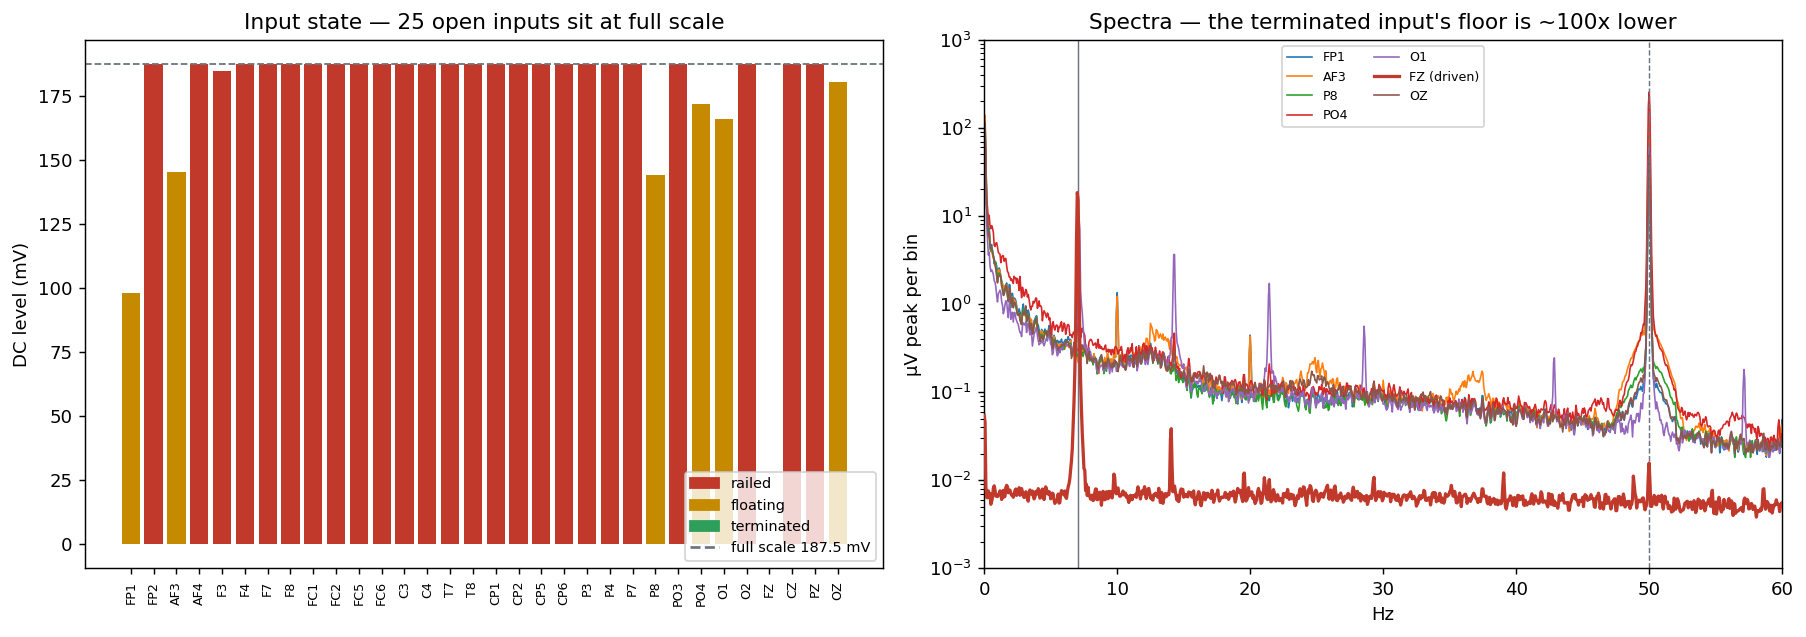
\includegraphics[width=\textwidth]{../results/crosstalk7_state.png}
\caption{Left: DC level per input. Twenty-five inputs sit exactly at full scale. Right:
amplitude spectra of the seven channels that are not saturated. The terminated channel (red)
has a noise floor roughly two decades below the floating ones and essentially no
\SI{50}{\hertz}; the floating channels carry \SIrange{3.5}{26.5}{\micro\volt} of mains and a
large low-frequency drift skirt.}
\end{figure}

\section{The driven channel}

Before asking about leakage, it is worth recording how the one properly connected channel
behaves, because it is the only clean characterisation of the amplifier in this dataset.

\begin{table}[h]\centering\small
\caption{Driven channel (FZ), \SI{179}{\second} record.}
\begin{tabular}{lrl}
\toprule
Amplitude & \SI{24.542}{\micro\volt} peak & \SI{17.354}{\micro\volt} rms \\
Amplitude stability & $24.05 \pm 0.03$~\uV & across 35 consecutive \SI{5}{\second} windows \\
Frequency & \SI{7.0226}{\hertz} & $+3235$\,ppm vs the nominal \SI{7}{\hertz} \\
THD ($2f$--$6f$) & \SI{0.22}{\percent} & \\
\SI{50}{\hertz} & \SI{0.0045}{\micro\volt} & \\
Noise, \SIrange{20}{45}{\hertz} & \SI{0.092}{\micro\volt} rms & \\
Noise-only ceiling at $f_0$ & \SI{0.066}{\micro\volt} & 95th pct of the null distribution \\
\bottomrule
\end{tabular}
\end{table}

Two remarks. First, \SI{0.092}{\micro\volt} rms over \SI{25}{\hertz} of bandwidth is consistent
with the ADS1299 datasheet's input-referred noise at gain 24, so the amplifier is behaving as
specified when its input is properly terminated. Second, the $+3235$\,ppm frequency offset is
the \emph{combined} error of the generator's timebase and the cap's sample clock and cannot be
attributed between them from this record alone. It is far too large for a crystal
($\approx$20\,ppm), so most of it belongs to one of the two oscillators being nominal-rather-than-
calibrated; a generator set to ``\SI{7}{\hertz}'' by a DIP switch is the more likely candidate.
Either way it is small enough not to matter for EEG band power, and large enough to destroy a
fixed-frequency fit (Section~\ref{sec:traps}).

\section{Two estimator traps}
\label{sec:traps}

\begin{figure}[h]\centering
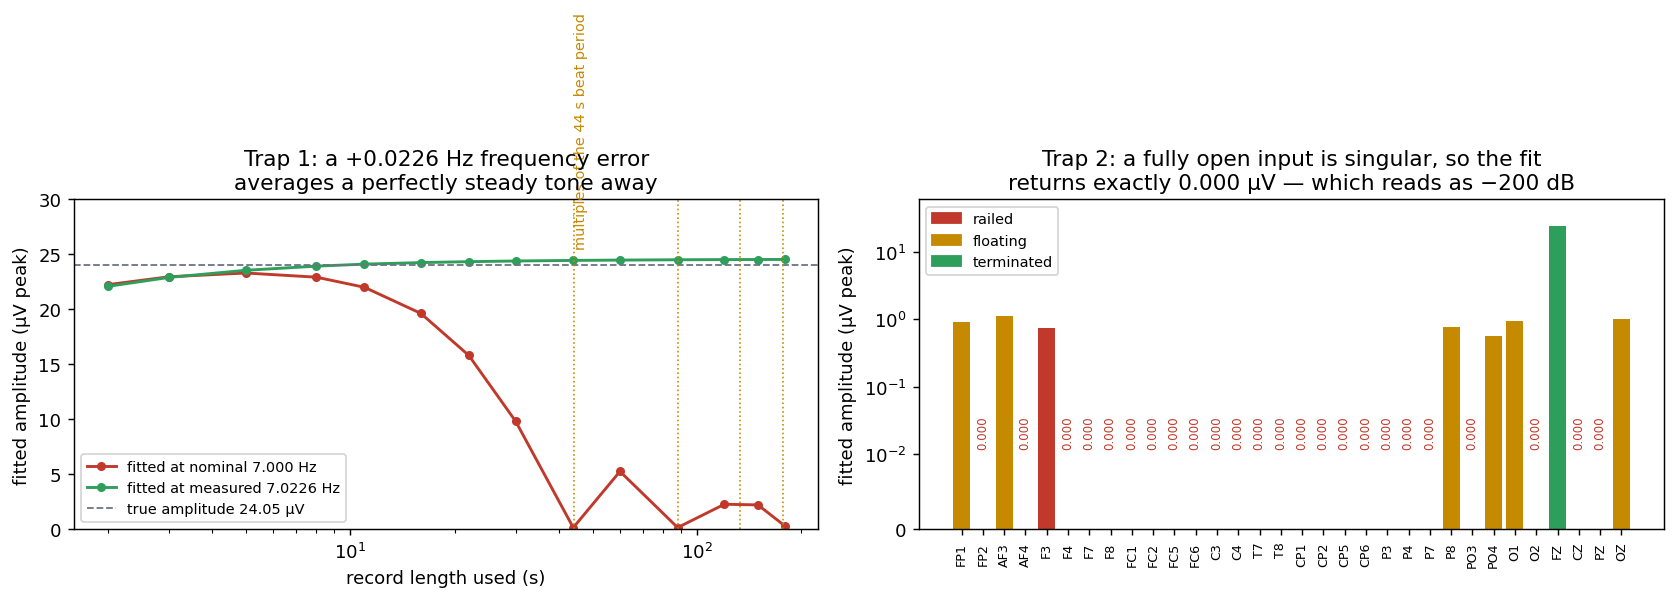
\includegraphics[width=\textwidth]{../results/crosstalk7_traps.png}
\caption{Left: the same steady \SI{24.05}{\micro\volt} tone, fitted at the nominal
\SI{7.000}{\hertz} (red) and at the measured \SI{7.0226}{\hertz} (green), as a function of how
much of the record is used. The red curve collapses at multiples of the \SI{44}{\second} beat
period. Right: fitted amplitude per channel. The 24 fully saturated inputs return exactly
\SI{0.000}{\micro\volt} because the least-squares system is singular --- which a
decibel conversion turns into $-200$\,dB, i.e.\ ``perfect isolation''.}
\end{figure}

\paragraph{Trap 1: fitting the nominal frequency.}
The tone is at \SI{7.0226}{\hertz}, not \SI{7.000}{\hertz}. A least-squares projection onto a
fixed \SI{7.000}{\hertz} sinusoid accumulates $2\pi \times 0.0226\,t$ of phase error, so over a
record spanning several \SI{44}{\second} beat periods the projection averages the tone away.
Measured on this record, the same signal reads:

\begin{center}\small
\begin{tabular}{lrrrr}
\toprule
Record length & \SI{11}{\second} & \SI{59}{\second} & \SI{179}{\second} & \SI{5}{\second} windows \\
\midrule
fitted at \SI{7.000}{\hertz} & \SI{21.84}{\micro\volt} & \SI{5.17}{\micro\volt} & \SI{0.31}{\micro\volt} & \SI{24.05}{\micro\volt} \\
fitted at \SI{7.0226}{\hertz} & \SI{24.5}{\micro\volt} & \SI{24.5}{\micro\volt} & \SI{24.54}{\micro\volt} & \SI{24.05}{\micro\volt} \\
\bottomrule
\end{tabular}
\end{center}

Read down the first row and the source appears to be dying exponentially across three
successive recordings. It is not: it is flat to $\pm\SI{0.1}{\percent}$ throughout. The fix is
to estimate the frequency once on the driven channel and use that same value for every channel,
so source and victims are measured on the same basis.

\paragraph{Trap 2: railed channels read as zero.}
For a channel pinned at a constant value the least-squares design matrix is singular and the fit
returns exactly \SI{0.000}{\micro\volt}. Converted to decibels that becomes $-200$, which
is indistinguishable in a results table from ``no crosstalk''. In the first run of this
measurement 24 channels landed in that state, and the worst-case crosstalk figure was then
computed across the six \emph{floating} channels only --- producing a headline
``$-\SI{4.8}{\deci\bel}$ worst-case crosstalk'' that was an artifact end to end. Open inputs must
be reported as unmeasurable, not as zero.

\section{Is the tone detectable on any other channel?}

An amplitude fit always returns a positive number. On a drifting channel with a
\SI{1}{\micro\volt}-scale noise skirt it returns roughly \SI{1}{\micro\volt} whatever frequency
is requested, so an absolute value alone establishes nothing. The test used here builds the null
from the channel's own noise: fit the amplitude at 75 frequencies spread over \SIrange{4}{10}{\hertz},
excluding $f_0$ and its first three harmonics, and ask what fraction of those null frequencies
return an amplitude at least as large as the one at $f_0$.

\begin{table}[h]\centering\small
\caption{Detection test, \SI{179}{\second} record, 75 null frequencies. \textbf{Bound} is the
null 95th percentile expressed in dB relative to the \SI{24.542}{\micro\volt}
source: the smallest leakage this channel could have revealed.}
\begin{tabular}{llrrrrrrl}
\toprule
Ch & State & $A(f_0)$ & null med & null p95 & $z$ & $p$ & Bound & Verdict \\
 & & \uV & \uV & \uV & & & dB & \\
\midrule
\textbf{FZ} & terminated & 24.542 & 0.027 & 0.066 & 1549.3 & 0.000 & $-51.3$ & \textcolor{good}{\textbf{tone present}} \\
\midrule
O1 & floating & 0.955 & 0.702 & 1.015 & 1.1 & 0.200 & $-27.7$ & not distinguishable \\
FP1 & floating & 0.899 & 0.773 & 1.257 & 0.4 & 0.427 & $-25.8$ & not distinguishable \\
OZ & floating & 0.995 & 0.855 & 1.382 & 0.5 & 0.427 & $-25.0$ & not distinguishable \\
AF3 & floating & 1.131 & 0.970 & 1.522 & 0.5 & 0.440 & $-24.1$ & not distinguishable \\
P8 & floating & 0.781 & 0.696 & 1.157 & 0.3 & 0.453 & $-26.5$ & not distinguishable \\
PO4 & floating & 0.576 & 0.583 & 0.927 & 0.2 & 0.507 & $-28.5$ & not distinguishable \\
\midrule
\multicolumn{9}{l}{25 railed channels: unmeasurable (no information at any frequency)} \\
\bottomrule
\end{tabular}
\end{table}

\begin{figure}[h]\centering
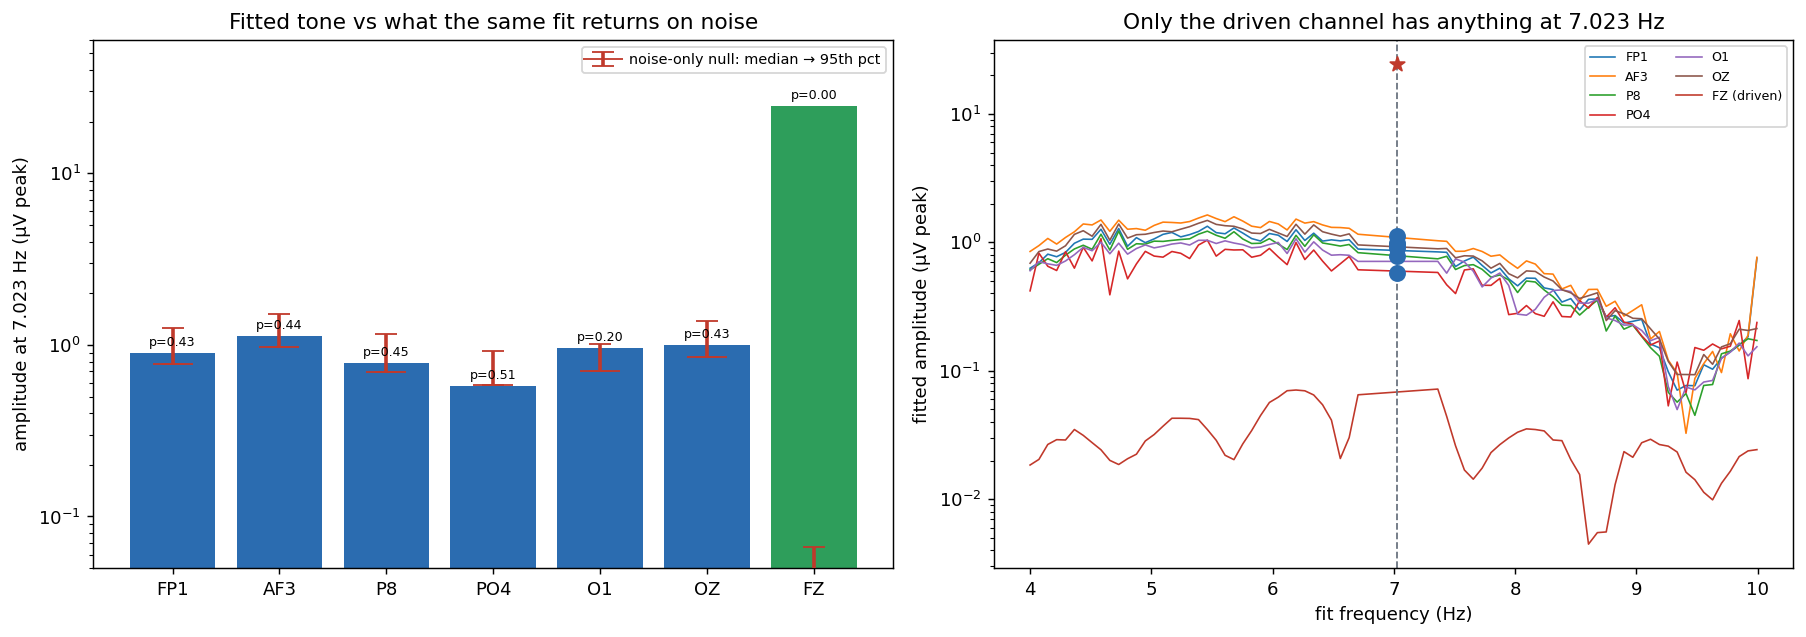
\includegraphics[width=\textwidth]{../results/crosstalk7_detection.png}
\caption{Left: fitted amplitude at $f_0$ per channel (bars) against the noise-only null median
and 95th percentile (red). Every floating channel's ``signal'' sits inside its own noise
distribution. Right: the same fit swept across frequency. The floating channels trace a smooth
$\sim$\SI{1}{\micro\volt} curve with \textbf{no feature at $f_0$}; the driven channel sits at
\SIrange{0.02}{0.07}{\micro\volt} everywhere except the single point at \SI{7.023}{\hertz}.
The right panel is the whole result in one image.}
\end{figure}

\section{Controls}

Three quantities looked, at first, like evidence of a shared coupling path. Each dissolves under
its own control.

\begin{figure}[h]\centering
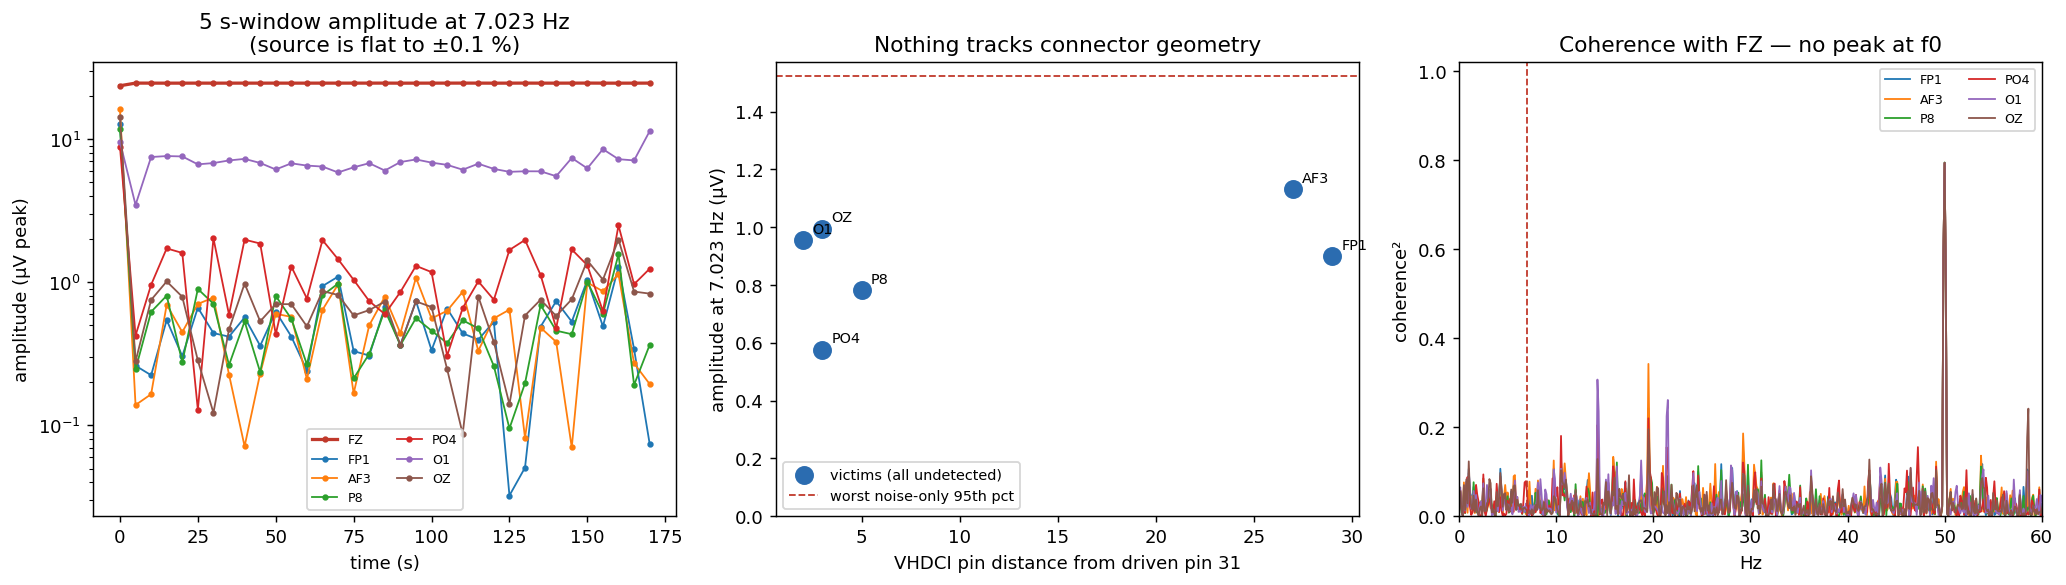
\includegraphics[width=\textwidth]{../results/crosstalk7_controls.png}
\caption{Left: \SI{5}{\second}-window amplitude at $f_0$; the source is flat, the floating
channels wander around \SI{1}{\micro\volt} with no relationship to it. Centre: amplitude against
VHDCI pin distance from the driven pin. Right: magnitude-squared coherence with the driven
channel --- no peak at $f_0$.}
\end{figure}

\paragraph{Phase clustering.} The six floating channels' phases at $f_0$ cluster within
$9.3^\circ$ (circular sd) of each other, which looks like one shared path. But the same
statistic computed at the 75 null frequencies has a median of $4.4^\circ$ --- \emph{tighter} ---
and $p = 0.787$. The floating inputs are phase-locked to one another at essentially every
frequency because they share the same ambient field (median pairwise broadband $r = 0.44$). A
tight cluster at $f_0$ is therefore expected under the null and carries no information.

\paragraph{Correlation with the source.} The decisive control. Broadband Pearson correlation
between the driven channel and each floating channel: $+0.0011$, $+0.0011$, $+0.0015$, $+0.0018$,
$+0.0021$, $+0.0022$. The driven channel is uncorrelated with every other channel in the cap.

\paragraph{Harmonics.} The floating channels return \SIrange{25}{45}{\percent} ``THD'', against
\SI{0.22}{\percent} on the source. Read naively this says the coupling path generates harmonics
and is therefore nonlinear. It says nothing of the kind: those are fits at $14$ and
\SI{21}{\hertz} to the same broadband noise that produced the fundamental, and a harmonic ratio
is meaningless while the fundamental itself is undetected.

\paragraph{Connector geometry.} Amplitude versus VHDCI pin distance from the driven pin 31 gives
$r = +0.47$ over $\Delta\text{pin} = 2$--$29$ --- weakly \emph{increasing} with distance, the
opposite of what ribbon lead-to-lead capacitance would produce. FP1 at $\Delta\text{pin}=29$
reads more than PO4 at $\Delta\text{pin}=3$. Consistent with there being no geometric coupling
to find.

\section{Replication: a second electrode, and a second sample rate}
\label{sec:repl}

One driven channel is one data point. The generator was moved to \textbf{FP1} --- VHDCI pin 2,
the opposite end of the connector from FZ's pin 31 --- and the measurement repeated, then
repeated again at \SI{1000}{SPS} instead of \SI{250}{}.

\begin{table}[h]\centering\small
\caption{Three independent sessions. \textbf{Src} is the driven amplitude, \textbf{drv floor}
the terminated channel's noise-only 95th percentile, \textbf{vic floor} the worst floating
channel's. \textbf{Bound} is vic floor in dB re. src --- the smallest leakage the session could
have revealed. \textbf{min $p$} is the most significant victim in that session.}
\begin{widetable}
\begin{tabular}{llrrrrrrrr}
\toprule
Session & Driven & Pin & Src \uV & $f_0$ Hz & drv floor & vic floor & Bound & min $p$ & $\max|r|$ \\
\midrule
FZ, \SI{250}{SPS}   & FZ  & 31 & 24.542 & 7.0226 & 0.066 & 1.522 & $-24.1$ & 0.200 & 0.002 \\
FP1, \SI{250}{SPS}  & FP1 & 2  & 24.554 & 7.0231 & 0.080 & 1.542 & $-24.0$ & 0.387 & 0.003 \\
FP1, \SI{1000}{SPS} & FP1 & 2  & 24.633 & 7.0233 & 0.065 & 1.914 & $-22.2$ & 0.400 & 0.004 \\
\bottomrule
\end{tabular}
\end{widetable}
\end{table}

\begin{figure}[h]\centering
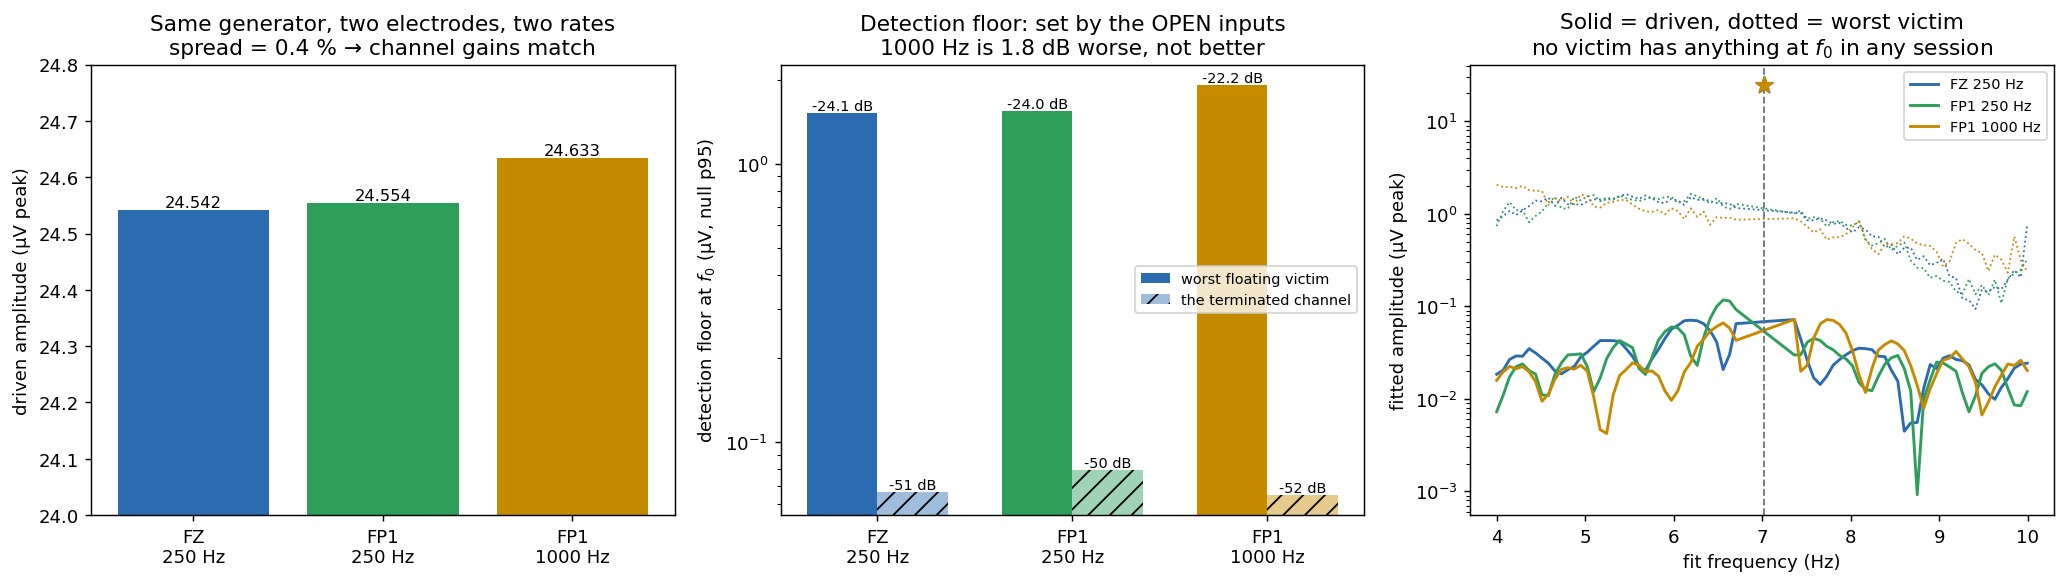
\includegraphics{../results/crosstalk7_replication.png}
\caption{Left: driven amplitude across the three sessions --- \SI{0.37}{\percent} total spread.
Centre: the detection floor, split into the terminated channel (hatched) and the worst floating
one. The gap between them, roughly \SI{27}{\deci\bel}, is the entire cost of leaving inputs
open. Right: the frequency sweep for all three sessions overlaid; solid is the driven channel,
dotted is that session's worst victim. Every dotted curve passes smoothly through $f_0$.}
\end{figure}

\paragraph{The result replicates.} No victim is detectable in any session
($p = 0.20$--$0.45$), the broadband correlation with the driven channel stays below $0.004$
in all three, and the bound lands within \SI{2}{\deci\bel} of the same place. Driving pin 2
and pin 31 --- opposite ends of the VHDCI --- gives the same answer, which also partly
discharges the ``move the driven channel'' item in Section~\ref{sec:protocol}: whatever
lead-to-lead coupling exists is below the floor at both ends of the connector.

\paragraph{A free calibration result.} The same generator into two different electrodes reads
\SI{24.542}{} and \SI{24.554}{\micro\volt} --- a \SI{0.05}{\percent} difference, and
\SI{0.37}{\percent} across all three sessions including the rate change. The datasheet specs
gain match between channels at \SI{0.2}{\percent} of full scale. Two channels is not a gain
survey, but as far as it goes, the channels agree with each other and with the part.

\paragraph{\SI{1000}{SPS} is worse, not better.} This was worth testing rather than asserting,
and the prediction held: the bound got \emph{worse} by \SI{1.8}{\deci\bel}, and the worst
victim's noise floor rose from \SI{1.542}{} to \SI{1.914}{\micro\volt} (\SI{+24}{\percent}).
The reason is that the detection floor at \SI{7}{\hertz} is set by the noise \emph{density}
there and by the total observation time ($\propto 1/\sqrt{T}$) --- neither of which a higher
sample rate improves. What a higher rate does change is that the ADS1299 averages less per
sample, so per-sample input-referred noise rises (the terminated channel's \SIrange{20}{45}{\hertz}
noise went \SI{0.090}{} $\to$ \SI{0.098}{\micro\volt} rms), and the board sends four times the
UDP traffic.

For this measurement \textbf{stay at \SI{250}{SPS} and record longer instead}: doubling the
record buys \SI{3}{\deci\bel}, quadrupling it buys \SI{6}{\deci\bel}, and it costs nothing but
time. A high sample rate would only be the right tool for a different question --- whether
coupling grows with frequency, which is the signature that separates capacitive from resistive
paths, and which needs a generator running at hundreds of hertz rather than at 7.

\section{What this does and does not establish}

\paragraph{Established.} Crosstalk from the driven channel into any measurable channel is below
\SI{-24.1}{\deci\bel} (worst channel AF3). The amplifier, when its input is terminated, has a
\SI{0.092}{\micro\volt} rms noise floor, \SI{0.22}{\percent} THD and negligible mains pickup.
No signal path was found between the driven channel and any other.

\paragraph{Not established.} Whether crosstalk is $-\SI{30}{\deci\bel}$ or
$-\SI{90}{\deci\bel}$. The bound is set by the \emph{victims'} noise, and 31 of them were
unconnected. A \SI{-24}{\deci\bel} bound is far too loose to be a hardware specification: a
\SI{50}{\micro\volt} alpha rhythm on one channel would be permitted to put \SI{3}{\micro\volt}
onto its neighbour, which would be a serious defect if real. Nothing here says it is real; the
measurement simply could not have seen it.

\paragraph{Also not established.} Any statement about coupling \emph{mechanism}. With no
detectable leakage there is nothing whose mechanism could be identified, and the phase,
harmonic and geometry patterns above are all noise.

\section{Protocol for a real crosstalk specification}
\label{sec:protocol}

\begin{enumerate}
\item \textbf{Terminate every unused input to generator ground.} This is the single change that
matters. It takes the victim noise floor from ${\sim}\SI{1.0}{\micro\volt}$ to
${\sim}\SI{0.07}{\micro\volt}$ and the bound from $-24$ to about \SI{-51}{\deci\bel}, on the
same \SI{179}{\second} record and the same source amplitude.

\item \textbf{Use the largest calibrator output.} At \SI{2000}{\micro\volt} instead of
\SI{24.5}{\micro\volt} the bound improves by a further \SI{38}{\deci\bel}, to roughly
\SI{-89}{\deci\bel} --- below any level that could matter for EEG.

\item \textbf{Measure the tone frequency; never assume the nominal.} One
\texttt{refine()} call on the driven channel, then fit every channel at that frequency.

\item \textbf{Report open inputs as unmeasurable.} Never let a singular fit become
\SI{-200}{\deci\bel}.

\item \textbf{Move the driven channel and repeat.} Drive a pin at one end of the connector, then
the middle, then the other end. If leakage ever becomes detectable, the dependence on
$\Delta\text{pin}$ separates ribbon lead-to-lead capacitance (falls off with distance) from a
shared REF/BIAS return (does not).

\item \textbf{Run the generator on battery} and keep leads short and twisted; a charger ties the
generator to mains earth and creates a ground loop through the amplifier.
\end{enumerate}

\section{How this compares to the silicon, and to normal practice}
\label{sec:lit}

Two questions were checked against external sources: is a railing open input normal, and is
the hardware acceptable on crosstalk?

\subsection*{The chip already has a crosstalk specification}

TI's ADS1299 datasheet (SBAS499C, Table 7.5 Electrical Characteristics) publishes the numbers
below. They are silicon-level typicals at gain 12, \SI{250}{SPS}, and the crosstalk figure is
the one that matters here.

\begin{table}[h]\centering\small
\caption{ADS1299 datasheet vs what this measurement could see.}
\begin{tabular}{llll}
\toprule
Parameter & Datasheet & Test condition & This measurement \\
\midrule
\textbf{Crosstalk} & \textbf{\SI{-110}{\deci\bel}} typ & $f_{\text{IN}} = 50/\SI{60}{\hertz}$
  & bound only, \SI{-24.1}{\deci\bel} \\
CMRR & \SI{-120}{\deci\bel} typ (\SI{-110}{} min) & $f_{\text{CM}} = 50/\SI{60}{\hertz}$ & not measured \\
THD & \SI{-99}{\deci\bel} & $f_{\text{IN}} = \SI{10}{\hertz}$ & \SI{-53}{\deci\bel} (generator-limited) \\
Input-referred noise & \SI{1}{\micro\volt\text{PP}} typ, \SI{1.35}{} max & \SI{0.01}{}--\SI{70}{\hertz}, gain 24
  & $\approx\SI{1.0}{\micro\volt\text{PP}}$ equivalent \\
Input bias current & \SI{\pm 300}{\pico\ampere} & $T_A = \SI{25}{\celsius}$ & --- \\
DC input impedance & \SI{1000}{\mega\ohm} & no lead-off & --- \\
Input capacitance & \SI{20}{\pico\farad} & & --- \\
\bottomrule
\end{tabular}
\end{table}

The comparison that matters: \textbf{the chip's own crosstalk specification is
\SI{-110}{\deci\bel}, and this measurement could only bound crosstalk at
\SI{-24}{\deci\bel}} --- \SI{86}{\deci\bel} short of being able to test it. That is not a
criticism of the hardware; it is a statement about what a measurement with 31 unconnected
inputs can resolve. Board layout and the VHDCI cable can of course add coupling on top of the
silicon, and that is exactly what a proper terminated-input measurement would look for.

The noise comparison is the one place where this record does reach the datasheet. Measured
\SI{0.092}{\micro\volt} rms over \SI{20}{}--\SI{45}{\hertz} (\SI{25}{\hertz} of bandwidth);
scaling a flat spectrum to the datasheet's \SI{0.01}{}--\SI{70}{\hertz} band gives
\SI{0.154}{\micro\volt} rms, and the conventional $6.6\sigma$ peak-to-peak conversion gives
\SI{1.02}{\micro\volt\text{PP}} against a datasheet typical of \SI{1}{\micro\volt\text{PP}} and a
maximum of \SI{1.35}{}. The extrapolation is mildly optimistic --- real amplifier noise has a
$1/f$ region below \SI{10}{\hertz} that a \SI{20}{}--\SI{45}{\hertz} measurement does not see,
so the true broadband figure will sit somewhat above \SI{1.02}{\micro\volt\text{PP}}. Even so, the
terminated channel is operating within the datasheet's typical-to-maximum window. The analog
front end is doing its job.

\subsection*{Railing on an open input is expected, and is documented as such}

The ADS1299 datasheet's pin table carries the instruction directly, as footnote (2) on every
\texttt{INxP}\slash\texttt{INxN}\ pin: \emph{``Connect unused analog inputs directly to AVDD.''}
Leaving them open is not a supported configuration.

The mechanism is in the same tables. An open input has no DC return, so the
\SI{\pm 300}{\pico\ampere} input bias current has nowhere to go but into the
\SI{20}{\pico\farad} input capacitance:
\[
\frac{dV}{dt} = \frac{I_{\text{bias}}}{C_{\text{in}}}
 = \frac{\SI{300}{\pico\ampere}}{\SI{20}{\pico\farad}} \approx \SI{15}{\volt\per\second},
\]
which drives the node into the supply rail within milliseconds. Twenty-five channels sitting at
exactly full scale is therefore not a fault --- it is the textbook response of this part to the
wiring used.

This also matches what the wider community reports for the same silicon. The OpenBCI Cyton
(also ADS1299-based) generates a steady stream of ``RAILED'' reports traced to floating or
poorly-referenced inputs, and the standard advice given there is that all EEG amplifiers behave
this way with floating pins because the front ends are extremely high impedance, and that the
diagnostic is to short channel, reference and bias together --- which should read close to zero
microvolts. That is precisely the state our FZ channel was in, and it read
\SI{0.092}{\micro\volt} rms.

\subsection*{Crosstalk is not a commonly published EEG specification}

Worth knowing when deciding what to compare against: commercial research EEG amplifiers
generally publish CMRR rather than channel-to-channel crosstalk. Brain Products' actiCHamp
quotes \SI{100}{\deci\bel} common-mode rejection per IEC 60601-2-26, and the IEC standard for
electroencephalographs is framed around amplitude accuracy, input dynamic range, input noise
and frequency response. So the ADS1299's \SI{-110}{\deci\bel} is a more specific number than
most amplifier vendors give, and there is no widely used pass/fail industry threshold for EEG
crosstalk to check this cap against. The practical threshold is the application one: leakage
should be far below the smallest signal of interest, and for MI work that means a
\SI{50}{\micro\volt} rhythm on one channel must not put a meaningful fraction of a microvolt
onto its neighbour --- roughly \SI{-40}{\deci\bel} or better as a working requirement.

\subsection*{Bottom line on hardware quality}

Nothing in this measurement indicates a crosstalk problem, and one channel's worth of evidence
says the analog front end meets its datasheet noise specification. But the measurement cannot
certify the cap: a \SI{-24}{\deci\bel} bound is looser than the \SI{-40}{\deci\bel} working
requirement, so ``no problem found'' is not yet ``verified good''. The terminated-input protocol
in Section~\ref{sec:protocol} closes that gap and costs one evening.

\section*{Sources}

\begin{itemize}\small
\item Texas Instruments, \emph{ADS1299-x Low-Noise, 4-, 6-, 8-Channel, 24-Bit ADCs for
Biopotential Measurements}, SBAS499C, rev.\ January 2017 --- Section 7.5 Electrical
Characteristics (crosstalk, CMRR, THD, input-referred noise, input bias current, input
capacitance, DC input impedance) and Section 6 Pin Functions (``Connect unused analog inputs
directly to AVDD'').
\url{https://www.ti.com/lit/ds/symlink/ads1299.pdf}
\item OpenBCI community forum, railed-channel threads on floating and poorly-referenced inputs
in the ADS1299-based Cyton board.
\url{https://openbci.com/forum/index.php?p=/discussion/3056/electrode-cap-all-channels-are-railed-resolved}
\item Brain Products GmbH, actiCHamp series specifications (CMR \SI{100}{\deci\bel} per
IEC 60601-2-26). \url{https://www.brainproducts.com/solutions/actichamp/}
\item IEC 60601-2-26:2012, \emph{Medical electrical equipment --- Part 2-26: Particular
requirements for the basic safety and essential performance of electroencephalographs}.
\url{https://webstore.iec.ch/en/publication/2637}
\end{itemize}

\section*{Data and reproduction}

\begin{center}\small
\begin{tabular}{ll}
\toprule
\cmd{recordings/calibrator/cal\_7hz\_180s.npz} & FZ driven, \SI{250}{SPS}, \SI{179}{\second} \\
\cmd{recordings/calibrator/cal\_7hz\_fp1\_250sps\_180s.npz} & FP1 driven, \SI{250}{SPS} \\
\cmd{recordings/calibrator/cal\_7hz\_fp1\_1000sps\_180s.npz} & FP1 driven, \SI{1000}{SPS} \\
\cmd{recordings/calibrator/cal\_7hz\_xt7hz\_60s.npz} & FZ, \SI{59}{\second} \\
\cmd{recordings/calibrator/cal\_7hz\_probe11s.npz} & FZ, \SI{11}{\second} \\
\cmd{results/crosstalk7.json}, \cmd{xt\_fp1\_250.json}, \cmd{xt\_fp1\_1000.json} & every number in this report \\
\bottomrule
\end{tabular}
\end{center}

\begin{shell}
python src/acquisition/crosstalk_analysis.py \
    recordings/calibrator/cal_7hz_180s.npz --freq 7 --json results/crosstalk7.json
\end{shell}

All recordings are raw \si{\micro\volt}, unfiltered, pre-CAR, all 32 channels retained.

\end{document}
